\chapter{Grundlagen der Sterilisation}

Nachfolgend werden wichtige Begriffe der Sterilisation definiert:
\begin{description}
	\item[Infektion:] Eindringen von Mikroorganismen in einen Makroorganismus und anschliessende Vermehrung der Mikroorganismen.
	\item[Desinfektion:] Gezieltes Abtöten oder Reduzieren von Mikroorganismen an und in kontaminierten Objekten; vom Objekt kann keine Infektion mehr ausgehen. Allgemeine Anforderung: Verminderung der Keimzahl um 4-5 Zehnerpotenzen.
	\item[Sterilisation:] Elimination aller Formen lebensfähiger Mikroorganismen, so dass der Zustand \textit{steril} erreicht wird. Die theoretische Wahrscheinlichkeit, dass sich ein lebensfähiger Mikroorganismus auf einem als \textit{steril} bezeichneten Produkt befindet, muss kleiner als eins in einer Million Produkten sein (EN 556-1). Typisch: Verminderung der widerstandsfähigsten Mikroorganismen um 12 Zehnerpotenzen.
\end{description}

\section{Mikroorganismen}

In diesem Abschnitt werden die gängigsten Mikroorganismen beschrieben.

\begin{description}
	\item[Bakterien] sind einzellige Kleinlebewesen (0.6 - 5 $\mu$m) mit eigenständigem Stoffwechsel (Antibiotika greifen Stoffwechsel an). Einige Bakterien bilden unter ungünstigen Umweltbedingungen Sporen (Erhöhte Resistenz gegen Hitze und Chemikalien).
	\item[Viren] sind keine Lebewesen (kein Stoffwechsel) und in den meisten Fällen Krankheitserreger. Können sich nur mit Hilfe einer Wirtszelle vermehren. Teilweise mit einer Hülle umgeben, welche sie vor dem Immunsystem schützt. Ist diese Hülle durchbrochen, können sie einfach unschädlich gemacht werden.
	\item[Pilze] besitzen im Unterschied zu Bakterien einen vollständigen Zellkern. Pilze sind aber nicht wie andere Pflanzen zur Photosynthese fähig. Etwa 300 der 100'000 bekannten Pilzarten sind für den Menschen krankheitserregend.
	\item[Prionen] sind kleinste, proteinhaltige infektiöse Partikel, welche virusähnliche Eigenschaften besitzen und dadurch äusserst resistent gegen Hitze, Strahlen, Chemikalien und Gase sind. Sie bestehen nur aus einem Protein und tragen keine Erbinformationen in sich. Deshalb sind sie keine Lebewesen sondern organische Gifte. 
\end{description}

Nachfolgend wird die Empfindlichkeit gegenüber Desinfektionsmittel / Sterilisation aufgelistet (resistent zuerst):
\begin{enumerate}
	\item Prionen
	\item Bakterielle Sporen
	\item Kleine unbehüllte Viren
	\item Mykobakterien
	\item Grosse, unbehüllte Viren
	\item Pilzsporen
	\item Bakterien und Hefepilze
	\item Behüllte Viren
\end{enumerate}

\section{Infektionsprävention}

Beim Anwender von Medizinprodukten werden re-Sterilisierbare Produkte (z.B. Instrumente beim Zahnarzt) oder Einmalgebrauchs-Produkte (z.B. Spritze) verwendet. Abbildung \ref{fig:insturmentenkreislauf} zeigt den relativ aufwendigen Prozess für die Sterilisation von wiederverwendbaren Instrumenten. Der Zahnarzt möchte sich aber nur mit dem rot eingekreisten Bereich befassen. Die anderen Prozessschritte werden deshalb oft von externen Dienstleistern durchgeführt. Diese Entwicklung führte zum Prozess der Einwegprodukte (Abbildung \ref{fig:einmalgebrauch}). Der Zahnarzt muss sich nur noch mit den letzten drei Schritten befassen.

\begin{figure}
	\centering
	\begin{subfigure}[b]{0.4\textwidth}
		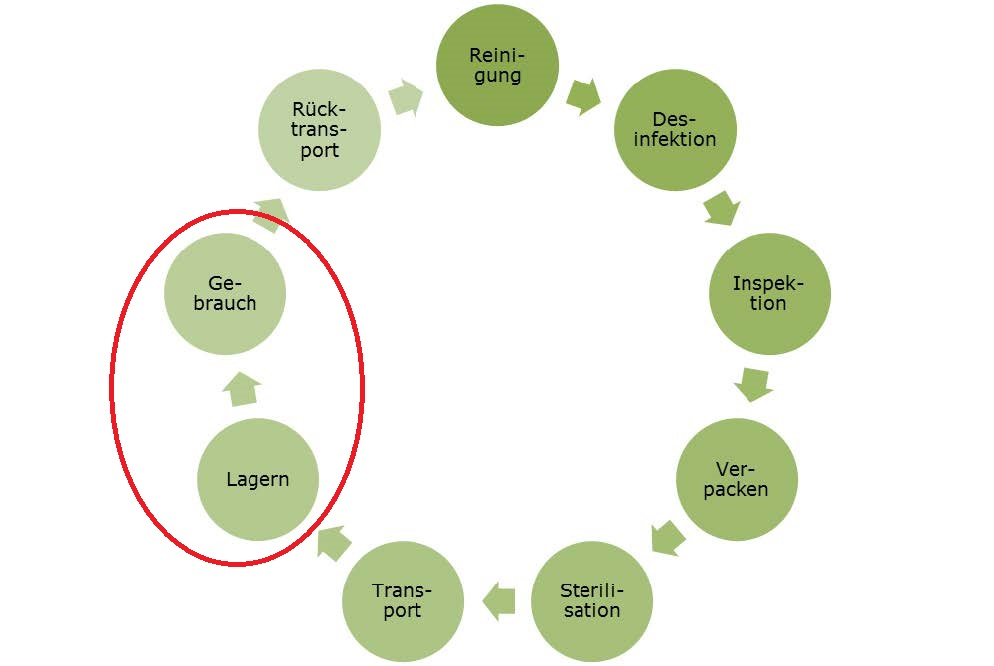
\includegraphics[width=\textwidth]{fig/insturmentenkreislauf}
		\caption[Wiederverwendbare Instrumente]{}
		\label{fig:insturmentenkreislauf}
	\end{subfigure}
	~ 
	\begin{subfigure}[b]{0.4\textwidth}
		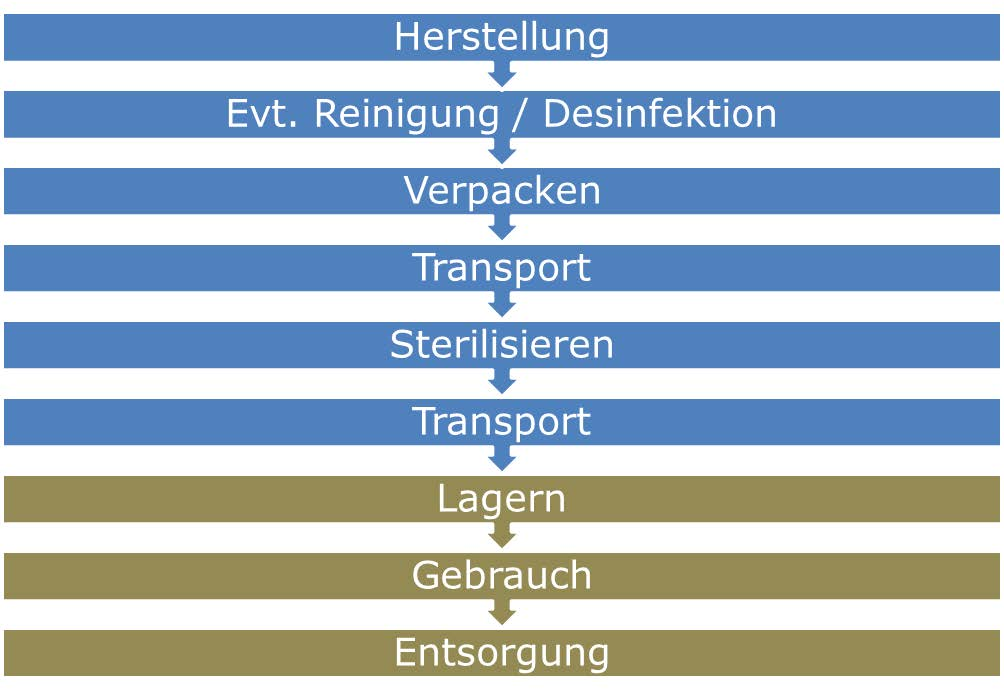
\includegraphics[width=\textwidth]{fig/einmalgebrauch}
		\caption{Einmalgebrauch}
		\label{fig:einmalgebrauch}
	\end{subfigure}

\end{figure}

\section{Sterilisationsmethoden}

Abbildung \ref{fig:sterilisationsmethoden} zeigt einen Überblick der gängigsten Sterilisationsmethoden. In den folgenden Abschnitten wird auf einige Verfahren detailliert eingegangen.

\begin{figure}
\centering
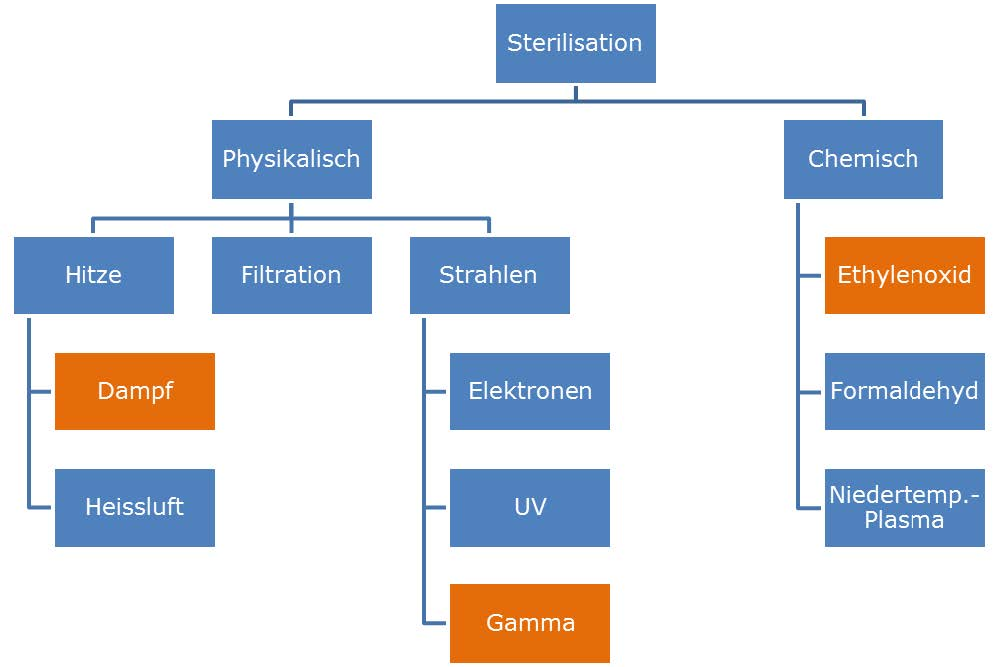
\includegraphics[width=0.7\linewidth]{fig/sterilisationsmethoden}
\caption{Sterilisationsmethoden}
\label{fig:sterilisationsmethoden}
\end{figure}

\subsection{Dampfsterilisation}

Überhitzter Wasserdampf kondensiert am Sterilisationsgut und gibt Kondensationswärme ab. Anhaftende Mikroorganismen werden durch die hohen Temperaturen (134ºC während 3 Minuten) inaktiviert. Dampf ist besser weil er eine höhere Feuchtigkeit hat. Bei trockener Luft bräuchte man viel höhere Temperaturen (>170ºC).

\begin{itemize}
	\item[+] Häufigste Sterilisationsmethode, insbesondere für wiederverwendbare Produkte
	\item[+] Ungefährliche und umweltverträgliche Stoffe (Wasser)
	\item[---] Hohe Temperaturen für viele Materialien ungeeignet. Insbesondere Kunststoffe
	\item[---] Dampf muss sämtliche Oberflächen erreichen. Kann insbesondere bei langen, sehr dünnen Kanülen schwierig sein
\end{itemize}

\subsection{Ethylenoxid-Sterilisation}

Ethylenoxid verbindet sich mit den Eiweissmolekülen (Proteinen) von Bakterien und Viren und bei ausreichender Befeuchtung auch von bakteriellen Sporen.

\begin{itemize}
	\item[+] Sehr geeignet für single-use Produkte aus Kunststoff
	\item[+] EO durchdringt viele Kunststoffe; erreicht damit auch kleine Hohlräume des Medizinproduktes
	\item[---] EO ist toxisch und krebserregend beim Einatmen
	\item[---] Praktisch nur in industriellen Anlagen verfügbar nicht geeignet für wiederverwendbare Produkte
	\item[---] Nach der Sterilisation: relativ lange Ausgasungszeiten
\end{itemize}

\subsection{Gamma-Sterilisation}

Die hochenergetischen Photonen zerstören die DNA und andere Zellstrukturen. Die Mikroorganismen werden damit abgetötet oder sind nicht mehr fähig zur Reproduktion.

\begin{itemize}
	\item[+] Sehr geeignet für single-use Produkte
	\item[+] Sterilisation bei Raumtemperatur
	\item[+] Gammastrahlung hat eine hohe Eindringtiefe
	\item[---] Gewisse Werkstoffe, auch Kunststoffe, reagieren mit der Strahlung
	\item[---] Praktisch nur in industriellen Anlagen verfügbar nicht geeignet für wiederverwendbare Produkte
	\item[---] Hohe Investitionskosten für die Sterilisationsanlagen
\end{itemize}